% !TEX root = ../main.tex




\usebackgroundtemplate{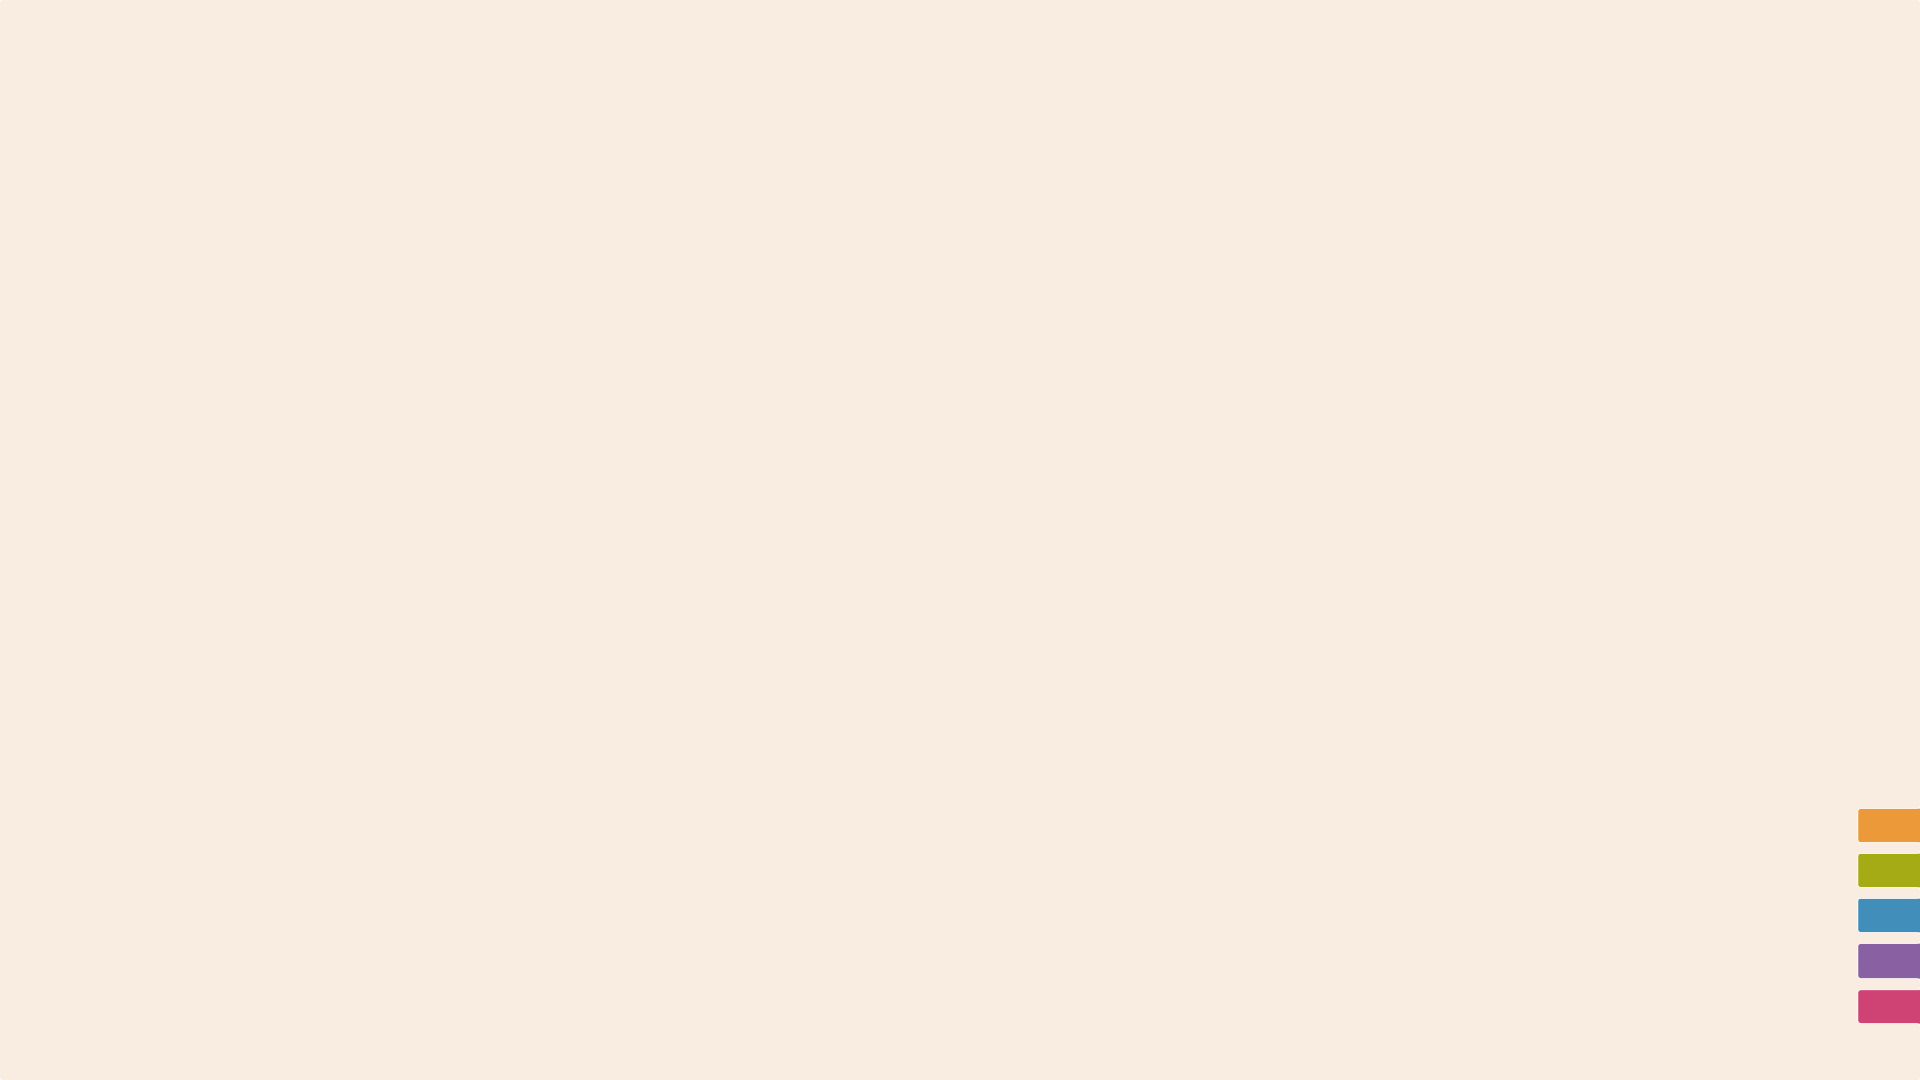
\includegraphics[width=\paperwidth,height=\paperheight]{achtergrond22n_FV}}



\begin{frame}{Inleidende oefening}
%\framesubtitle{}
\begin{figure}
\href{run:./media/Cowcattlejumpingintowatertocrosstheriver.webm}{%
\includegraphics[height=\textheight-3\baselineskip]{vlcsnap-2024-09-30-08h26m35s430}
}
\end{figure}
\end{frame}

\note[itemize]{%
\item Eenvoudigere setting om een snelheidsvector mee te associ\"eren dan bij de kromme baan in het vorige voorbeeld. Nu zijn de vectoren constant in de tijd. Bij het vorige voorbeeld is het dus de vraag: hoe ga je niet-constante snelheden defini\"eren \dots?
\item Snelheid afleiden via totale afgelegde weg te delen door de tijd. Eerst de grote en zien dat het niet de som van de afzonderlijke snelheden is. Baan is rechte. Daaruit dat snelheid vector moet zijn; grootte is afstand na 1 seconde. 
}


\begin{frame}
\frametitle{Inleidende oefening}
\framesubtitle{}
Een buffel tracht loodrecht een \SI{300}{m} brede rivier over te steken met een snelheid van \SI{1,00}{m/s}. De stroomsnelheid bedraagt \SI{1,50}{m/s}.
\begin{enumerate}
		\item In welke tijd bereikt de buffel de overzijde?
		\item Hoever drijft de buffel af?
		\item Wat is de `snelheid' van de buffel?
		%\item Construeer de snelheidsvectoren en bereken de grootte van de resulterende snelheid.
	\end{enumerate}
\end{frame}

%\note[itemize]{%
%\item 
%\item 
%}

\begin{frame}
\frametitle{Inleidende oefening}
\framesubtitle{}
\begin{figure}
	%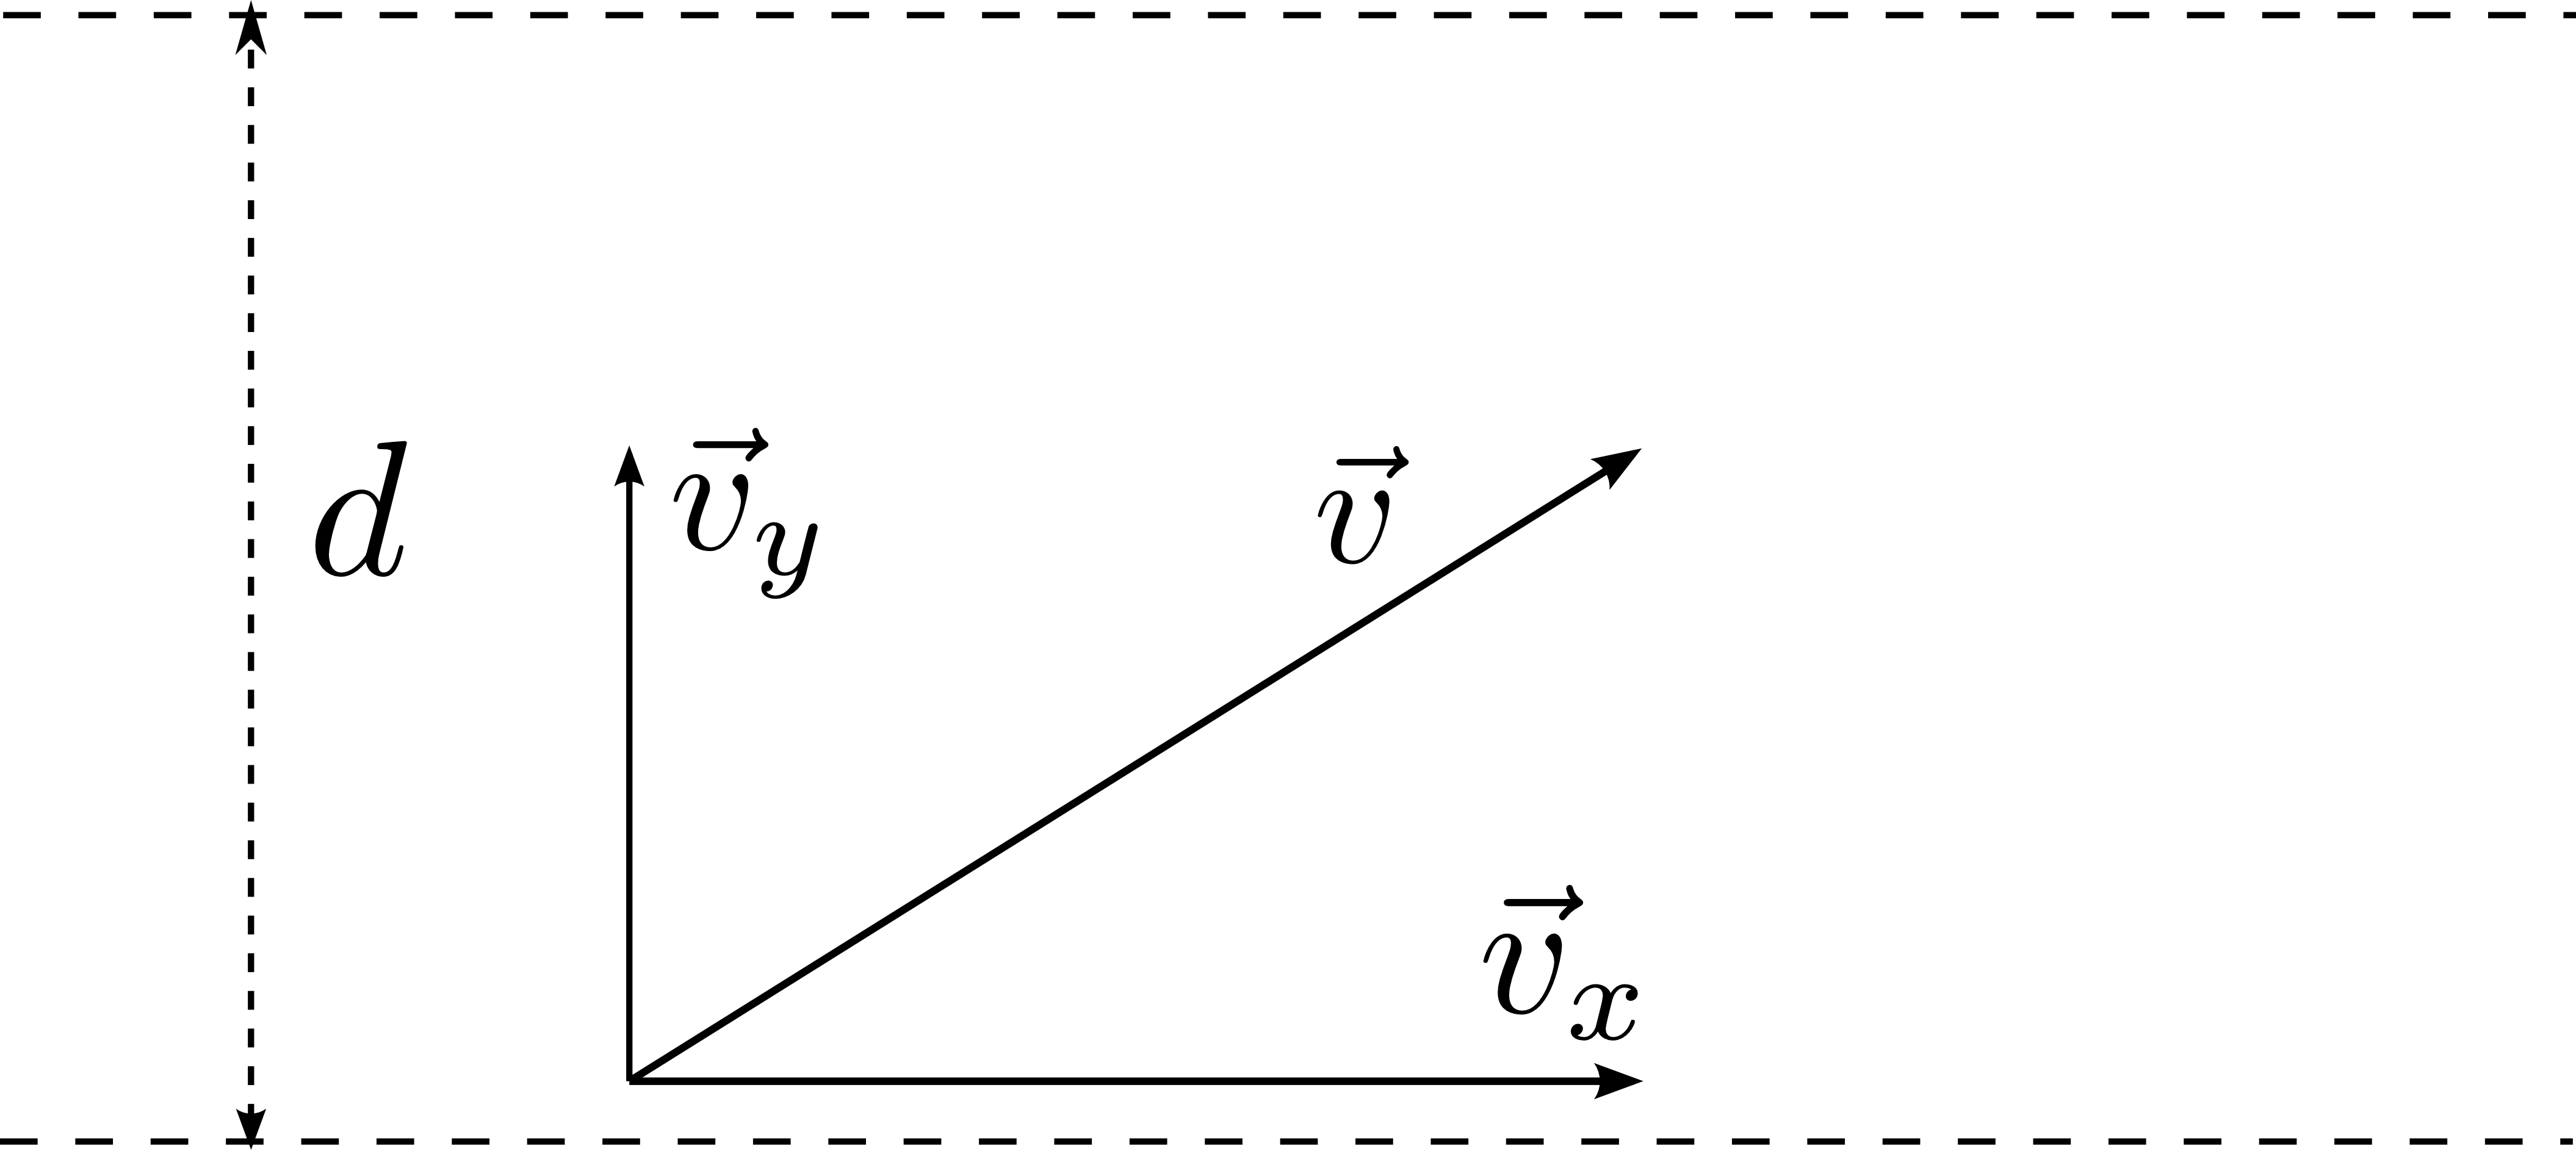
\includegraphics[height=\textheight-3\baselineskip]{4p49}
	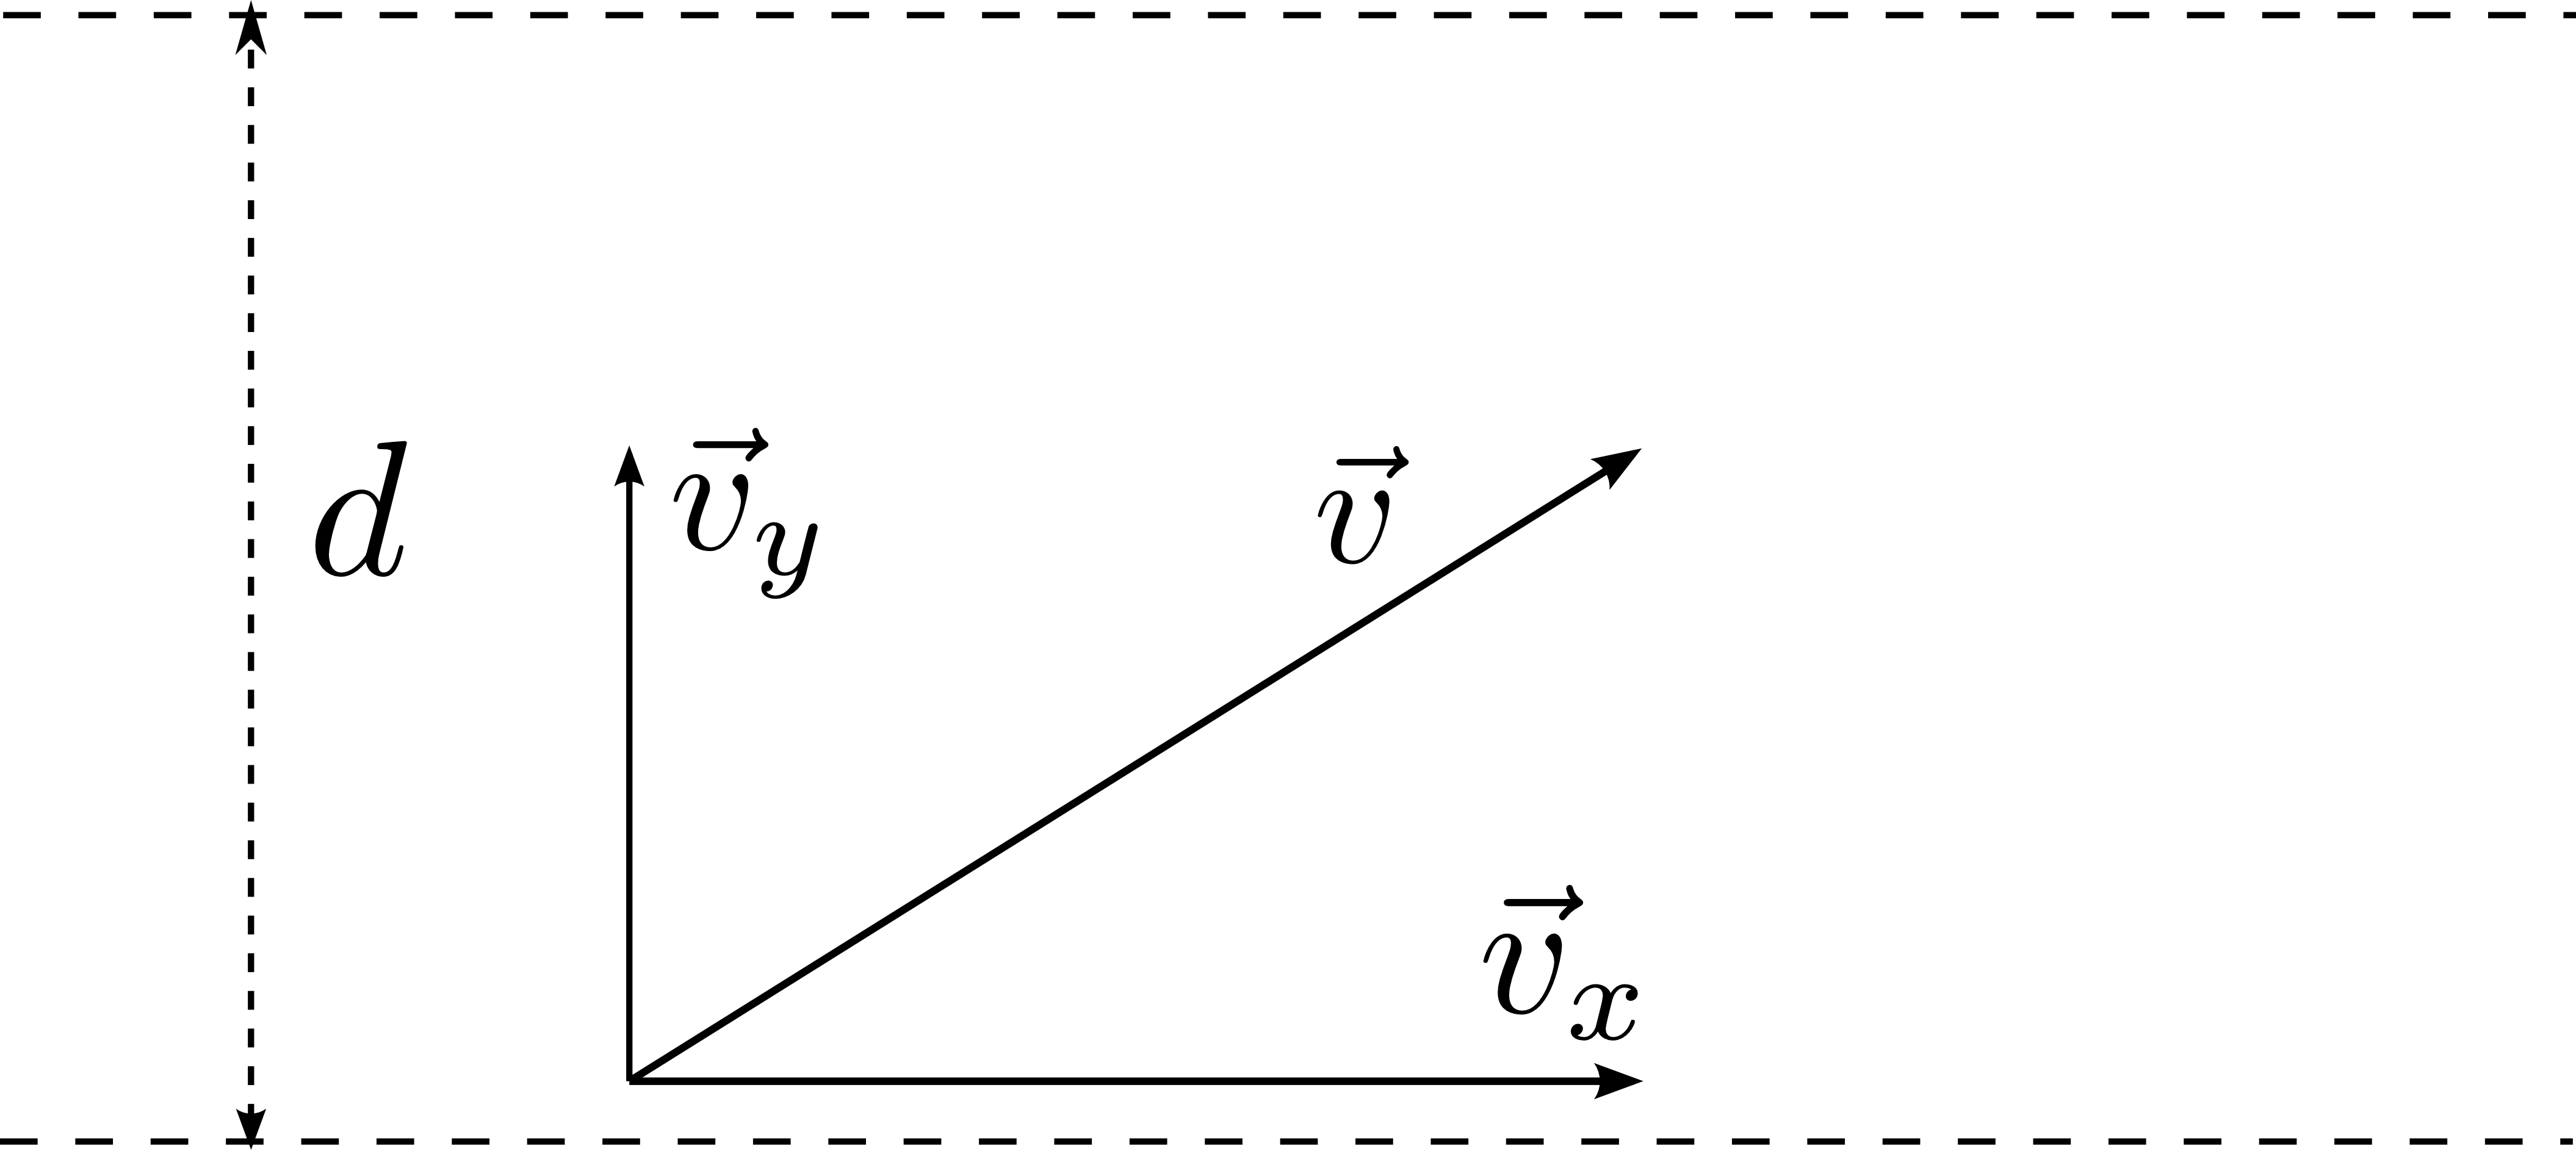
\includegraphics[width=\textwidth]{4p49}
\end{figure}
\end{frame}

%\note[itemize]{%
%\item 
%\item 
%}





\usebackgroundtemplate{
\includegraphics[width=\paperwidth,height=\paperheight]{achtergrond22n}}






\begin{frame}{Inleiding}
%\framesubtitle{}
\begin{figure}
\href{run:./media/ProjectilefromaMovingTruckDemo.webm}{%
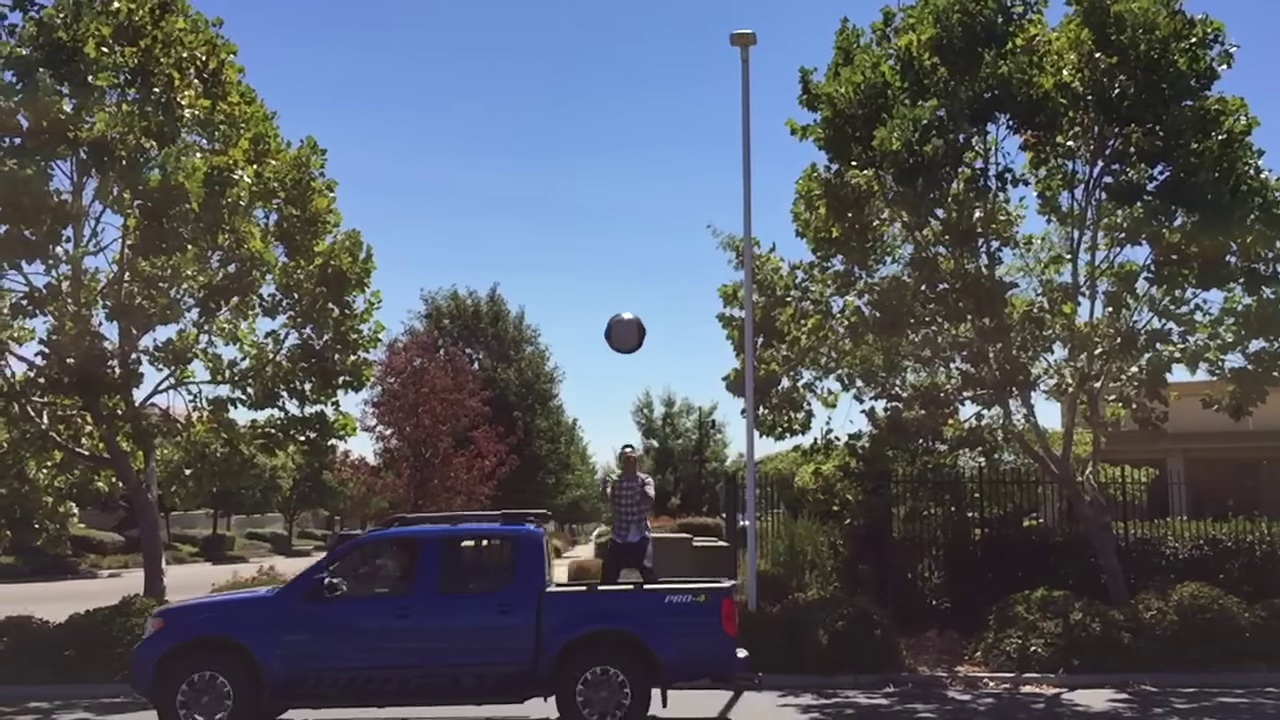
\includegraphics[height=\textheight-3\baselineskip]{vlcsnap-2022-09-21-21h28m34s708}
}
\end{figure}
\end{frame}

\note[itemize]{
\item Baan: twee dimensies nodig om die te beschrijven
\item Beweging beschrijven: splitsen we de beschrijving van de beweging op in twee 1-dimensionale bewegingen, nl. in de $x$- en de $y$-richting. Wat is de snelheid waarmee de bal vooruit gaat? (Zoals de auto) Wat is het snelheidsverloop in verticale zin? (ref stelsel in de auto zetten)
\item Referentiestelsel bepaalt het beeld dat wij hebben van de beweging. Positie en snelheid zijn relatieve begrippen
\item Nood aan vectoren! Antwoord op de vraag met wat voor grootheid we de snelheid kunnen beschrijven. En de versnelling ...?
\item Wrijving verwaarlozen
}








%\begin{frame}
%\frametitle{Inleiding}
%\framesubtitle{}
%\begin{figure}
%	\includegraphics[height=\textheight-3\baselineskip]{sworp_kuleuvencursus}
%	%\includegraphics[width=\textwidth]{}
%\end{figure}
%\end{frame}
%
%%\note[itemize]{%
%%\item 
%%\item 
%%}

